% arara: pdflatex
% arara: showfile
\documentclass{beamer}

\usepackage{tikz}
\usepackage{bbding}
\usepackage{tikzlings}
\usetikzlibrary{overlay-beamer-styles}
\setbeamertemplate{navigation symbols}{}

\setbeamercolor{background canvas}{bg=gray}
\usepackage{xfp}
\ExplSyntaxOn
\let\intmodnn\int_mod:nn
\ExplSyntaxOff

\begin{document}
\begin{frame}[plain]
\begin{tikzpicture}[remember picture,overlay]
% Background image
\node[at=(current page.center), anchor=center]{%
	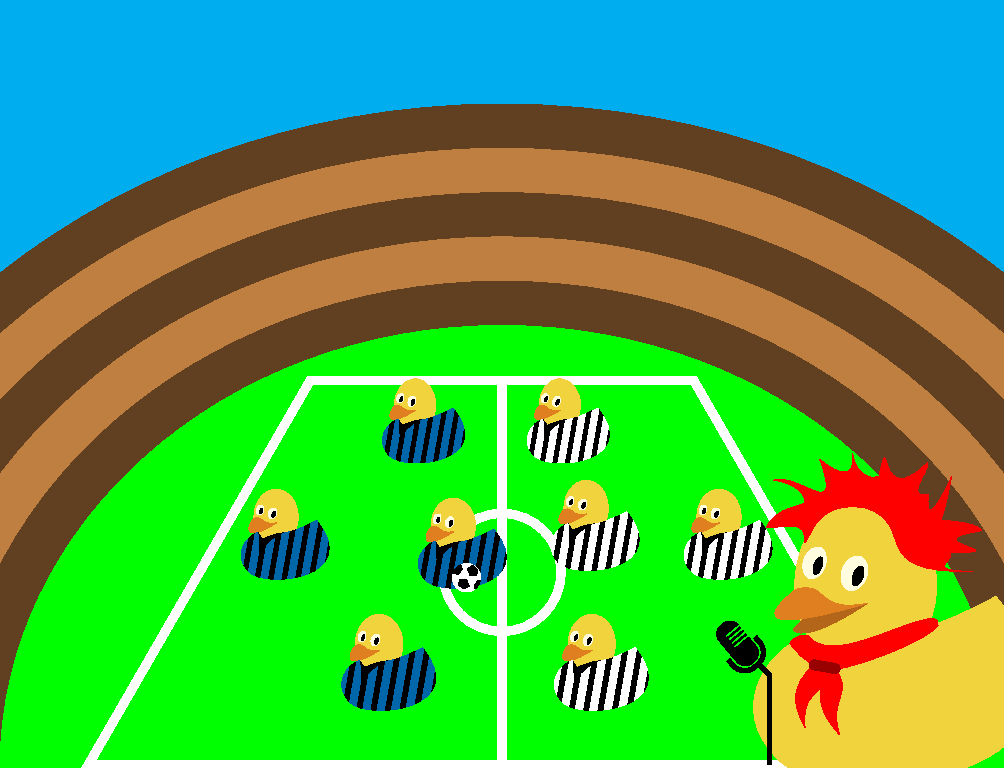
\includegraphics[%height=\paperheight
		width=\paperwidth]{soccerfield.pdf}
};	
\foreach \x in {1,...,60}{
	\node[at=(current page.center), anchor=center] {
		\ifnum \intmodnn{\thepage}{6} > 2
		\includegraphics<+>[width=\paperwidth]{Gianna_close}%
		\else
		\includegraphics<+>[width=\paperwidth]{Gianna_open}%
		\fi%
	};	
}
\end{tikzpicture}
\end{frame}
\end{document}